\documentclass{article}
\usepackage[utf8x]{inputenc}

\usepackage{enumitem}
\usepackage{xcolor}
% \AddToHook{shipout/before}{%
%   \ifodd\value{page}
%     \pagecolor{blue!10!white}% Odd page colour (light blue)
%   \else
%     \pagecolor{red!10!white}% Even page colour (light red)
%   \fi
% }


\usepackage{geometry}
\geometry{letterpaper, margin=1in}

\providecommand{\tightlist}{%
  \setlength{\itemsep}{0pt}\setlength{\parskip}{0pt}}

\usepackage{adjustbox}
\usepackage[hyphens]{url}
\usepackage{lineno,hyperref}
\modulolinenumbers[5]

%% APA style
\usepackage{graphicx}
\usepackage{caption}

\definecolor{almond}{rgb}{0.94, 0.87, 0.8}
\usepackage{pagecolor}
\usepackage{afterpage}

\begin{document}
\pagestyle{empty}
\thispagestyle{empty}
\pagecolor{gray!30}

\begin{figure}[h]
\begin{adjustbox}{minipage=[c]{\textwidth-10mm},margin= 5mm 5mm 5mm 10mm, frame=1pt, bgcolor=almond,env=center}%
%\begin{adjustbox}{varwidth=\textwidth,bgcolor=almond,margin=3mm {\abovecaptionskip} 3mm 3mm, frame=1pt }
\begin{center}
 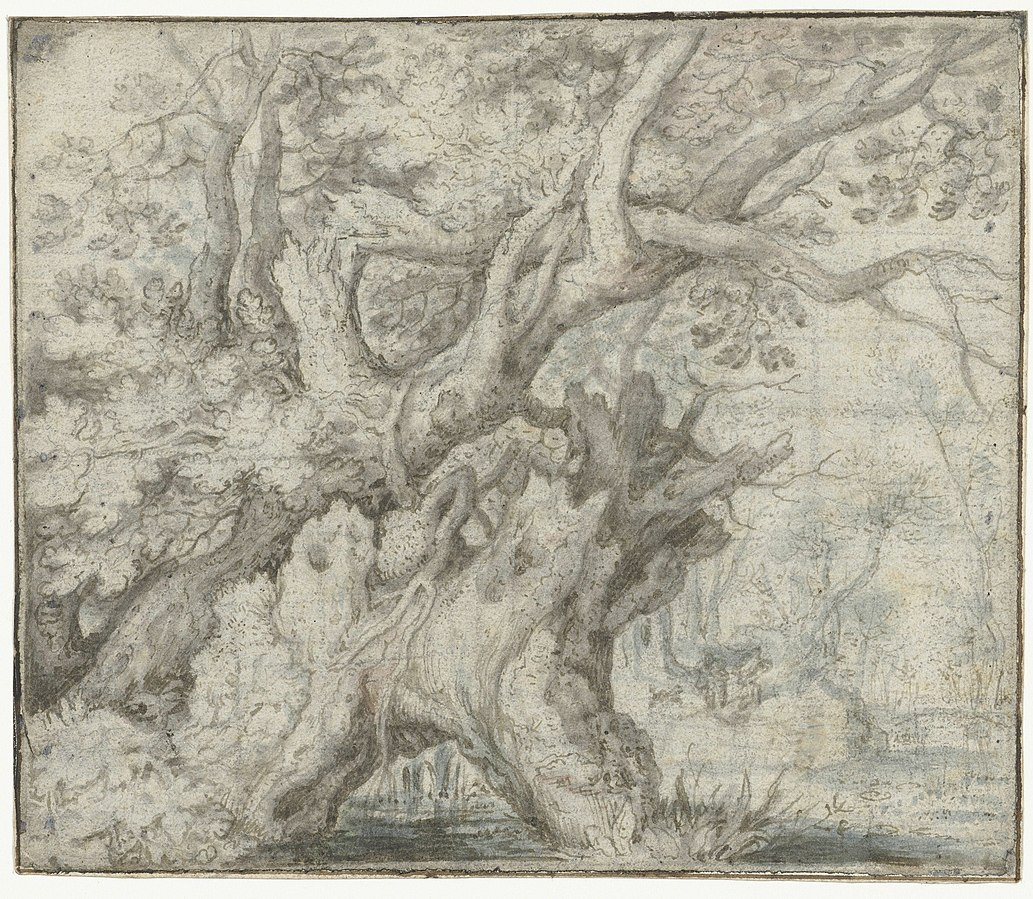
\includegraphics[trim=5mm 8mm 5mm 8mm,clip,width=.5\paperwidth]{water_chart.jpg}
\end{center}

\begin{center}
\begin{minipage}[t]{0.7\paperwidth}

\medskip
{\huge Project Action Review}
\bigskip

\Large\raggedright
\textbf{Context} Work in progress.\newline
\textbf{If} we are working on something together
BUT we might lose momentum;\newline
\textbf{Then} use a review template to think about our progress.  Questions like the following can be asked at any point in a project, and provide a momentary record of perspectives which can be analysed later.

\medskip

\begin{enumerate}[noitemsep,topsep=0pt,parsep=0pt,partopsep=0pt]
\item \emph{Review the intention: what do we (did we) expect to learn or make together?}
\item \emph{Establish what is happening: what and how are we learning?}
\item \emph{What are some different perspectives on what’s happening?}
\item \emph{What did we learn or change?}
\item \emph{What else should we change going forward?}
\end{enumerate}

\end{minipage}
\end{center}
\caption*{Image: Knoestige bomen aan het water (Gnarled trees by the water). Public Domain via Wikimedia Commons.\newline \url{https://commons.wikimedia.org/wiki/File:Knoestige_bomen_aan_het_water_Knoestige_bomen_bij_het_water_en_jagers,_RP-T-1975-46.jpg}}
\end{adjustbox}
\end{figure}



\end{document}